
%-----------------------------------------------------------------------------
\chapter{Epistatic GWAS analysis\label{ch:gwas}}
%-----------------------------------------------------------------------------

%---
\section{Preface}
%---

%---
\section{Introduction}
%---

Genetic studies aim to discover how a phenotype of interest, such as height or disease risk, is affected by genetic background. A typical study can detect millions of genetic variants \cite{clarke2011basic}, but only a few of them may be linked to the disease. For instance so far there are roughly 80 variants assumed to contribute to Type 2 diabetes risk, and these variants were discovered through in many different association studies in different populations. In this context, ``variant prioritization" means to select a small but meaningful set of genetic variants from a sequencing study in order to perform further validation. 

Genome wide association studies (GWAS) are powerful variant prioritization techniques that find variants that have significant statistical association to a phenotype or disease of interest \cite{visscher2012five}. Most GWAS have focused on finding association of single variants, often with moderate success. Recently, methods known as ``burden tests", have allowed to analyze groups of variants within a gene or group of genes (e.g. a pathway) \cite{wu2011rare}.

Epistasis is broadly defined as ``the study of genetic interaction" \cite{gao2010classification}. The basics for these ideas have been proposed almost a hundred years ago by Bateson (1909) and Fisher (1918), who coined the term to denote a ``statistical deviation of multilocus genotype values from an additive linear model for the value of a phenotype" \cite{gao2010classification}. The underlying idea is that, since most proteins perform their function(s) through physical interactions with other proteins, mutations in interacting loci can dramatically increase or decrease phenotype risk compared to individual mutations \cite{cantor2010prioritizing}. There is evidence of such gene-gene interactions are involved in complex diseases, such as Alzheimer, where results have been consistently replicated \cite{combarros2009epistasis}. Recently, the importance of epistatic interactions was highlighted as they are suspected to be the main reason GWAS have justified only a small portion of phenotypic variance \cite{zuk2012mystery}, a problem known as ``missing heritability" \cite{manolio2009finding}. 

Although simple statistical models exist to capture epistatic interactions \cite{de2013emerging}, they run into severe multiple hypothesis testing issues when applied on a genome-wide scale.  Given that the number of candidate ``pairs of variants" is quadratic in the number of variants considered, significance p-value thresholds have to be adjusted accordingly, thus diminishing statistical power. For this reason and due to lack of sequencing cohorts large enough to detect these interactions, the application of epistatic models to sequencing studies has not been widespread. There is no clear consensus on the required sample size to detect interaction, depending on phenotypic effect size and variant’s allele frequency some estimates assume in the order of 10,000 to 500,000 cases \cite{jostins2013using} to be required. Such cohorts are now becoming feasible due to improvements and cost reductions in sequencing technology.

In this work we propose methodologies to prioritize pairs of variants from a sequencing or genotyping experiment by combining genome wide association studies with epistatic interaction models. Performing GWAS using epistatic models is a challenging problem for several reasons: i) interaction models are by definition non-linear \cite{gao2010classification}; ii) analyzing pairs of loci in a sequencing experiment requires great computational power and efficient algorithms \cite{phillips2008epistasis}; and iii) multiple testing correction can render association tests underpowered for all but very large cohorts \cite{gao2010classification,phillips2008epistasis}. These problems are aggravated by the fact that there is no consensus of what genetic interaction means \cite{mani2008defining}, which is reflected in the difficulty to find a unified model \cite{phillips2008epistasis,mani2008defining}.

Interacting proteins can be identified experimentally through several types of approaches (Yeast-Two-Hybrid, Protein fragment complementation assay, Glutathione-s-transferase, Affinity purification coupled to mass spectrometry, Tandem affinity purification, etc. \cite{shoemaker2007deciphering}) and large databases of protein-protein interactions are now available for human \cite{shoemaker2007deciphering}. Nevertheless, these methods predict the interaction between proteins and may not discern the exact residues where such proteins interact. Furthermore, it is estimated that up to 80\% large of the human protein-protein interactions remains unknown \cite{venkatesan2009empirical}. 

Issues related to coverage and finding interacting residues can be addressed using computational predictions of either pairs of interacting proteins or interacting residues \cite{shoemaker2007deciphering}. A type of approaches that has been gaining popularity recently is one that makes use of the plethora of genomic sequences available for species other than human in order to discover evolutionary evidence of selective pressure on individual residues to identify active sites an  interaction interface \cite{marks2012protein}. Interacting residues and their neighbors may then be subject to compensating epistasis, where a mutation at a residue in one protein may be compensated by another mutation at a residue in the second protein \cite{pazos1997correlated}. Assuming that evolutionary pressure acts on both interaction sites simultaneously, co-occurring compensatory mutations can happen with higher probability than non-compensatory ones. In light of this hypothesis, we can use statistical methods on multiple sequence alignments (MSA) of proteins from different organisms to find coevolving / co-occurring mutation sites by means of statistical methods that prioritize loci having higher probability of epistatic interaction. There are several examples of coevolution acting both within a protein (e.g. N-terminal and C-terminal domains in PKG protein \cite{goh2000co} or the GroES-L chaperoning system \cite{ruiz2013coevolution}, $\alpha$ and $\beta$ haemoglobin subunits \cite{pazos1997correlated}), and between interacting proteins (e.g. G-protein coupled receptors and protein ligands \cite{goh2000co}).

Many methods exist to find putative interaction sites based on evolutionary evidence (see \cite{de2013emerging} for a review). One of the simplest methods for inferring co-evolution uses mutual information ($MI$) between two loci \cite{marks2012protein} in a multiple sequence alignment ($\mathcal{M}_{sa}$) of two proteins. However, methods based on correlation or mutual information are known to have systematic bias (e.g. due to phylogeny \cite{de2013emerging}, or sequence heterogeneity problems \cite{weigt2009identification}). More sophisticated methods, such as DCA \cite{morcos2011direct}, PSICOV \cite{jones2012psicov} or mdMI \cite{clark2014multidimensional} try to overcome these biases, but are usually not suitable for GWAS scale analysis for two main reasons: i) these methods require multiple alignments of a very large number of sequences (from $400$ to $25L$, where $L$ is the length of the protein \cite{clark2014multidimensional}), such depth is not usually available at whole genome scale; and ii) these methods are computationally demanding (e.g. running for minutes or even days for each interacting pair of proteins being considered), making them unsuitable for GWAS scale analysis involving millions of variants. Furthermore, a recent study shows that overall agreement between methods is not high (65\% or less) and prediction power is quite low (only 6\% of he ``top scoring pairs" are real interactions) \cite{clark2014multidimensional}.

The focus of the previously mentioned methods (such as DCA, PSICOV) is to pinpoint the amino acids involved in protein interactions using only MSA data. In our analysis, the goal is slightly different, since we want to detect interacting variants that might have impact on a phenotype by combining information MSA and GWAS information (sequencing and phenotype data). For this, we use a ``two tier" analysis: i) MSA information modulates our priors of putatively interacting residues, and ii) genotype information from a sequencing study to perform statistical association between genotype and phenotype. Since we have additional information and we don’t fully rely on MSA information, our method can trade off speed for accuracy when increasing priors of putative interacting sites. This tradeoff allows us to engineer faster algorithms that can be applied to genome wide scale datasets.

In a nutshell, our method uses recently computed 100-way vertebrate genome alignments to calculate interaction posterior probabilities for any given pair of residues in human proteins. This is achieved by contrasting the likelihood of the observed pair of alignment columns under a joint substitution model that models dependencies between interacting sites, and a null model of independent evolution.  These posterior probabilities are then used as priors to modulate the evidence of epistatic interaction derived from GWAS data. 

\textbf{We apply our approach to the analysis of ... and show that it succeeds at finding...}

%---
\section{Methods}
%---

Our epistatic GWAS pipeline (Figure \ref{fig:gwaspipeline}) consists of the following steps: i) select ``interacting amino acids" from protein structural data (PDB); ii) use a multiple sequence alignment, phylogentic tree and ``interacting amino acids", to estimate our model parameters; iii) annotate variants using SnpEff \cite{cingolani2012program} and filter out non-coding or synonymous variants using SnpSift \cite{cingolani2012using}; iv) pre-calculate all matrix exponentials $P(t_i+t_j)$ and $P_2(t_i+t_j)$; v) filter out pairs of variants that are not suitable for the analysis (have zero interaction terms, linearly dependent genotype coefficients, very low Hardy Weimberg p-values, etc.); vi) for each remaining pair of variants, calculate logistic regression; vii) filter out if logistic regression p-value is over a threshold; viii) calculate $LL(MSA)$ using Felsestenin’s algorithm; ix) calculate Bayes Factor, using Laplace approximation.

\begin{figure}
    \centering
    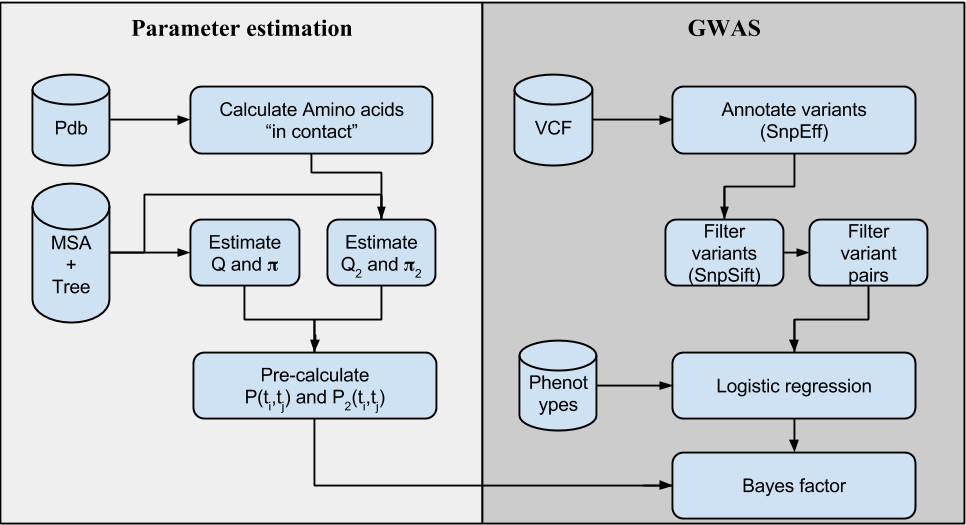
\includegraphics[width=12cm]{gwas_epistasis_pipeline.png}
    \caption{Complete pipeline}
    \label{fig:gwaspipeline}
\end{figure}

\subsection{Markov model}

Viewing evolutionary mechanisms in light of Markov models makes the models tractable \cite{yang2006computational}. This is also a reasonable hypothesis, because we can assume that a sequence at time $t$ will ``mutate" into a new sequence at time $t+1$ without influence from past sequences. Note that we use sequences of amino acids ($a_i \in \{a_1, ..., a_{20}\}$) instead of genomic coordinates for simplicity. For each amino acid in the sequence, there is a probability of mutating into another amino acid \cite{felsenstein2004inferring} that is given by a probability transition matrix $P(t)$. This matrix $P(t)$ obviously depends on the time because given a longer period of time, there is a higher chance of a random mutation. For small times $P(t)$ can be approximated by a constant rate matrix $Q$, such that $P(t) = e^{tQ}$. We can decompose the expression $e^{Qt} = U e^{\Lambda t} U^-1$, where $\Lambda$ is a diagonal matrix of all eigenvalues ($\lambda_i$). It can be shown that the all eigenvalues are negative, thus that matrix is stable \cite{yang2006computational}.

Given a simple phylogenetic tree, where two sequences ($s_i$ and $s_j$) are descendant from $s_k$ at times $t_i$ and $t_j$ respectively, we can estimate transitions frequencies from amino acid $i$ to amino acid $j$ simply by counting the number of events in the sequence alignment ($c_{i,j}$). Assuming ``time symmetry", the frequency is $f_{i,j}(t_i+t_j) = \frac{c_{i,j} + c_{j,i}}{n}$, where $n$ is the total number of transitions. It can be shown that $f$ is related to the transition probability $f_{i,j}(t_i+t_j) = \pi_i p_{i,j}(t_i+t_j)$, hence we can estimate the probability matrix as $\hat{P(t_i+t_j) = \hat{F}_{i,j}(t_i+t_j) \Pi^-1}$, where $\Pi$ is a diagonal matrix consisting of stationary distribution of amino acids $\pi_i = P(a_i)$ which satisfy detailed balance condition $ P(t) \bar{\pi} = \bar{\pi}$. Estimating the rate matrix $Q$ requires calculating the log of a matrix $\hat{Q}_(t_i+t_j) = log[ \hat{P}_(t_i+t_j) ]$.

Using the previous equations, we can estimate $\hat{Q}(t_i+t_j)$, the rate matrix for two sequences that diverged from their root node $k$ at times $t_i$ and $t_j$. If the phylogenetic tree has $N$ leaf nodes, we can calculate $\hat{Q}(t_i+t_j)$ for all leaf nodes combinations. Taking into account the estimation error, the equation becomes $\hat{Q}(t_i+t_j) = Q + \epsilon_{i,j}$, where $\epsilon_{i,j}$ is an error matrix. Under the assumption that the mean error is zero, we can approximate the rate matrix by the calculating an average of all estimates: $\hat{Q} = \frac{1}{N * (N-1)/2} \sum_{i < j} \hat{Q}_(t_i+t_j) = \sum_{t_i+t_j} \frac{1}{t_i+t_j} log[ \hat{P}_(t_i+t_j) ]$.

This model can easily be extended to account for co-evolutionary hypothesis by taking into account transitions of interacting amino acid pairs, instead of single amino acids. In an epistatic model, the new rate matrix $Q_2$ is a $400x400$ matrix (instead of $20x20$). In order to estimate this epistatic transition matrix, we use pairs of amino acids that are assumed to be interacting. We define a pair of amino acids to be ``interacting" if there is PDB information indicating that any pair of atoms has a distance of 3 Angstrom or less \cite{burger2010disentangling}.

Given a multiple sequence alignment $\mathcal{M}_{sa}$, and the corresponding phylegentic tree $\mathcal{T}$, and the transition matrix $Q$, we would like to calculate the likelihood of the data $L(\mathcal{M}_{sa}, \mathcal{T} | Q)$. Imagine having a tree with two nodes. Let $P(L_k|a)$ denote the probability of all nodes below $k$, assuming events in branches are independent and using Markov's reversibility, we can show that \cite{durbin1998biological}

\begin{eqnarray*}
P(L_k |  a_k ) 
& = & \sum_{a_i, a_j}{ P(a_k | a_i, a_j, t_1, t_2) P(L_i, L_k | a_i, a_j)  }
% = \sum_{a_i, a_j}{ P(a_k | a_i, t_1) P(L_i | a_i) P(a_k | a_j, t_2) P( L_k | a_j) } \\
= \sum_{a_i, a_j}{ P(a_i | a_k, t_1) P(L_i | a_i ) P(a_j | a_k, t_2) P( L_k | a_j) }
\end{eqnarray*}

This algorithm for propagating likelihoods from leaf nodes to the root is known as Felsestein's algorithm \cite{felsenstein2004inferring}. We can compute the likelihood of the whole $\mathcal{M}_{sa}$ as the product of the likelihoods of the root nodes for all positions in the alignment. This assumes independence of amino acids at each position, which is a necessary simplification in order for the problem to be tractable.

Using the rate matrices ($Q$ and $Q_2$) we compute a likelihood ratio by means of Felsestein’s algorithm calculated using .

\[
lr(\mathcal{M}_{sa}) = \frac{P(L_{i,j} | Q_2)}{P(L_i | Q) P(L_j | Q_)}
\]

where the denominator assumes that the amino acids $i$ and $j$ evolve independently. 

Both the Markov epistatic model and Felsenstein’s algorithm calculation require multiple sequence alignment and the corresponding phylogenetic tree. In order to use these algorithms at genome wide scale, we speed up computations by pre-calculating all matrix exponentials ($P(t_i+t_j)$) using parallelized code to make use of all available CPUs. Precomputed matrices are valid only if the phylogenetic tree remains constant across the whole genome, thus the values $t_i+t_j$ do not change. Another optimization (``constat-tree caching") is to cache likelihood values for parts of the phylogenetic tree where all nodes have the same amino acid values, this optimization results in speedup only if the phylogenetic tree remains constant throughout the genome.

\subsection{GWAS model}

Given $N_S$ samples (individuals), we use the standard notation for phenotypes and code them as $d_s=1$ meaning that the individual $s$ is affected by disease and $d_s=0$ if the individual is "healthy". Let $\bar{d} = [d_1, ..., d_{N_s}]$ be a phenotype vector and $g_{s,i} \in \{0,1,2\}$ a genomic variant for sample $s$, loci $i$ (we assume there are $N_V$ variants). A logistic model of disease risk \cite{balding2006tutorial} is

\[
p_{s,i} = P( d_s | g_{s,i} ) = \phi( \theta_0 + \theta_1 g_{s,i} + \theta_2 c_{s,1} + \theta_4 c_{s,2} + ... ) = \frac{1}{1 + e^{\theta_0 + \theta_1 g_{s,i} + \theta_2 c_{s,1} + \theta_4 c_{s,2} + ...}} = \phi( \bar{\theta}^T \bar{g}_{s,i})
\]

where $\phi(\cdot)$ is the sigmoid function, $c_{s,1}, c_{s,2}, ... $ are covariates for each individual $s$ (this covariates usually include sex, age and eigenvalues form population structure analysis \cite{price2006principal}), $\bar{g}_{s,i} = [ 1, g_{s,i} , c_{s,1}, c_{s,2}, ... , c_{s,N_C} ]$, and $\bar{\theta} = [\theta_1, \theta_2, ..., \theta_m] $. The parameters $\bar{\theta}$ are obtained by solving the maximum likelihood equation

\[
L( \bar{\theta} ) = \prod_{s=1}^{N_S}{ P( d_s | \bar{\theta}, g_{s,i} ) } = \prod_{s=1}^{N_S}{ p_{s,i}^{d_s} (1-p_{s,i})^{1-d_s} } = \prod_{s=1}^{N_S}{ \phi( \bar{\theta}^T \bar{g}_{s,i})^{d_s} (1-\phi( \bar{\theta}^T \bar{g}_{s,i}))^{1-d_s} }
\]

where $p_{s,i} = P( d_s | \bar{\theta}, g_{s,i} )$ is the probability of individual $s$ disease outcome, given a genomic variant.

Using this model, we have two hypotheses: i) the null hypothesis, $H_0$, assumes that genotype does not influence disease probability (i.e. $\theta_1 = 0$). ii) the alternate hypothesis, $H_1$, assumes that the genotype does influences disease probability. We can compare these two hypothesis using a likelihood ratio test $\Delta = L( \bar{\theta}_{alt} | H1 ) / L( \bar{\theta}_{null} | H0 ) $ which, according to Wilk's theorem, has a $\chi^2_1$ distribution, so we can easily calculate a p-value.

Next, we extend the logistic model to accommodate interacting loci. For an individual (sample $s$), we model interactions between two genetic loci $i$ and $j$, having genotypes $g_{s,i}$ and $g_{s,j}$, by extending the logistic model with $N_{cov}$ covariates $c_{s,j}$ as

\begin{eqnarray*}
P( d_s | g_{s,i},g_{s,j}, H_1) & = & \phi[ \theta_0 + \theta_1 g_{s,i} + \theta_2 g_{s,j} + \theta_3 (g_{s,i} g_{s,j}) + \theta_4 c_{s,1} + ... + \theta_m c_{s,N_{cov}} ] 
%\\
%\Rightarrow  P( d_s | g_{s,i},g_{s,j}, H_1) & = & 
= \phi( \bar{\theta}^T \bar{g}_{s,i,j}) )
\end{eqnarray*}

where $\bar{g}_{s,i,j} =  [1, g_{s,i}, g_{s,j}, ( g_{s,i} g_{s,j}), c_{s,1}, c_{s,2}, ..., c_{s,N_{cov}} ]^T$. An implicit assumption in this equation is that $g_{s,i}$ and $g_{s,j}$ are not correlated (i.e. in an LD-Block). This can be enforced by limiting the application of this model to variants either in different chromosomes or over ~1M bases apart. The null hypothesis $H_0$ assumes that variants act independently

\begin{eqnarray*}
P( d_s | g_{s,i},g_{s,j}, H_0) & = & 
\phi[ \theta_0' + \theta_1 g_{s,i} + \theta_2 g_{s,j} + \theta_3 c_{s,1} + ... ] 
%\\
%\Rightarrow  P( d_s | g_{s,i},g_{s,j}, H_1) & = & 
= \phi( \bar{\theta}^T \bar{g}_{s,i,j}' )
\end{eqnarray*}

where $\bar{g}_{s,i,j}' =  [1, g_{s,i}, g_{s,j}, c_{s,1} , c_{s,2}, ..., c_{s,N_{cov}} ]^T$. Since these models are not nested (i.e. $H_0$ is not included in $H_1$), we cannot directly apply Wilks theorem.

Logistic regression was implemented using several different algorithms to reach the desired performance. The fastest convergence is obtained using Iterative Reweighted Least Squares (IRWLS \cite{daubechies2010iteratively}) and Broyden–Fletcher–Goldfarb–Shanno algorithm (BFGS \cite{broyden1970convergence}) with some code optimizations. In most cases IRWLS converges faster, so it was selected as the default implementation in our analysis.

Another way to compare the null hypothesis to the alternative hypothesis, is using Bayesian formulation \cite{kass1995bayes,wakefield2009bayes}

\begin{eqnarray*}
P(H_1 | \mathcal{D}) & = & \frac{ P( \mathcal{D} | H_1) P(H_1) }{ P(\mathcal{D}) } = \frac{ \int{ P(\mathcal{D} | \theta , H_1) P( \theta | H_1)  d\theta } }{ P(\mathcal{D}) }  \\
\Rightarrow  \frac{ P(H_1 | D)  }{ P(H_0 | D)  } & = & \frac{ \int{ P(\mathcal{D} | \theta , H_1) P( \theta | H_1)  d\theta } }{\int{ P(\mathcal{D} | \theta , H_0 ) P( \theta | H_0)  d\theta } } \frac{ P(H_1) }{ P(H_0)  }  
=  B_F \frac{ P(H_1) }{ P(H_0)  }
\end{eqnarray*}

Where $B_F$, the ratio of the two integrals, is the Bayes factor. Using a Bayesian formulation has two main advantages: i) the hypothesis are automatically corrected for model complexity since Bayesian Information Criteria (BIC) is implicitly within Bayes Factors \cite{kass1993bayes}, and ii) we can compare non-nested models. The Bayes factor for the epistatic model becomes:

\begin{eqnarray}\label{eq:bf2}
B_F = \frac
{ \int{ \prod_{s=1}^{N_S}{ \phi( \bar{\theta}^T \bar{g}_s)^{d_s} [ 1-\phi( \bar{\theta}^T \bar{g}_s) ]^{1-d_s} } P( \bar{\theta} | H_1)  d\theta } }
{ \iint{ \prod_{s=1}^{N_S}{ 
\phi( \bar{\theta}^T \bar{g}_{s,i}) 
\phi( \bar{\theta'}^T \bar{g}_{s,j} ) )^{d_s} 
[ 1-\phi( \bar{\theta}^T \bar{g}_{s,i}) \phi( \bar{\theta'}^T \bar{g}_{s,j} ) ]^{1-d_s} } 
P( \bar{\theta} | H_0) 
P( \bar{\theta}' | H_0)  
d\theta d\theta' } }
\end{eqnarray}

Unfortunately, calculating Bayes factors is not trivial and most of the times there are no closed form equations. Calculating the integrals using numerical algorithms is possible, but  imposes a significant computational burden thus rendering unfeasible for large datasets, such as GWAS data, even using large computing clusters. We can approximate the integrals using Lapace's method  \cite{kass1995bayes}. If $g(x)$ has a minimum at $x_0$, it can be shown that

\begin{eqnarray*}
\int{e^{\lambda g(x)} h(x) dx} & \simeq & h(x_0) e^{\lambda g(x_0)} \sqrt{\frac{2 \pi}{\lambda g''(x_0)}} \\
\end{eqnarray*}

The multivariate case, for $\bar{x} \in \Re^d$, is analogous, we just need a Hessian matrix instead of a second derivate of $g(\cdot)$

\begin{eqnarray}\label{eq:laplace}
\int{e^{\lambda g(\bar{x})} h(\bar{x}) d\bar{x}} & \simeq & h(\bar{x}_0) e^{\lambda g(\bar{x}_0)} 
\left( \frac{2 \pi}{\lambda} \right)^{d/2} \left[ \frac{\partial^2 g(\bar{x}) }{\partial \bar{x} \partial \bar{x}^T} \right] ^{-1/2}
\end{eqnarray}

Using equation \ref{eq:laplace} we can try to approximate the complex integrals in equation \ref{eq:bf2} by the transformation $L(\bar{\theta}) = e^{\ell(\bar{\theta})}$, where $\ell(\cdot)$ is the log-likelihood of the data. So, we can use Laplace approximation by using Eq.\ref{eq:laplace}, at the point of the maximum likelihood.

We need to calculate the Hessian matrix in Eq.\ref{eq:laplace}. Fortunately, for logistic models, we can make a few simplifications. Considering that $L(\bar{\theta}) = \prod_{s=1}^{N_S}{ \phi( \bar{\theta}^T \bar{g}_s)^{d_s} [ 1-\phi( \bar{\theta}^T \bar{g}_s) ]^{1-d_i} }$, it can be shown that for genotype terms

\begin{eqnarray*}
\frac{ \partial^2 \ell(\bar{\theta}) }{ \partial\theta_i \partial\theta_j } 
= \sum_s{ g_{s,i} g_{s,j} p_s (1-p_s) } 
\end{eqnarray*}

Using analogous derivation for the covariates, we can find an analytic form of the Hessian, which completes the Laplace approximation formula.

It is easy to see that the computational burden for detecting detection of pairs of interacting genetic loci affecting disease risk is significantly larger than a standard (single variant) GWAS study. A priori all pairs of variants should are analyzed thus significantly increasing the number of statistical tests. This also reduces statistical power since the required p-value significance level would orders of magnitude smaller. A naive approach would estimate that if a typical genetic sequencing study has $10^6$ variants a GWAS on epistatic variants would square that number of statistical tests, thus p-values required for significance would be in the order of $0.05 / (10^6)^2 = 5 \cdot 10^{-14}$. 

Fortunately these numbers can be refined significantly. First, we only annotate variants and focus on non-synonymous ones, so we can filter out non-coding and synonymous variants. Second, if two variants are very low frequency, there are high chances that their interaction term $(g_{s,i} g_{s,j})$ is zero for all samples, thus there is no point on calculating the logistic regression since in the epistatic model $\theta_3$ would always be zero and we can skip these variant pairs. Third, if the variants and the epistatic term $[g_{s,i}, g_{s,j}, g_{s,i} g_{s,j}]$ are linearly dependent, the logistic regression result will be meaningless, so we can safely skip such variant pairs. Fourth, if one of the variants has high allele frequency respect to the other, all non-zero epistatic terms may lie in the same positions as non-zero genotypes from the low frequency variant. This causes the logistic regression to artificially inflate the coefficients of the low frequency variant and the epistatic term thus creating an artificially high association (low p-value). So we filter out these variant pairs as well. Finally, we filter out all variants having Hardy-Weinberg p-value of less than $10^-6$, since these variants also artificially inflate the logistic regression coefficients. After all filters have been applied, using real life data of over 1 million variants, the number of variant pairs to be analyzed is less than 50 millions, as opposed to the naive estimation of $~10^{12}$ variant pairs. By means of the z-score relationship \cite{goodman1999toward}, we set the significance threshold for $50$ million at $log_{10}[BF] =  8.0$ .

Calculating Bayes factors involves using prior parameter distributions. In order to estimate the distributions, we run the logistic regression fitting analysis and plot the parameter distributions for different levels of significance. As expected most parameters have unimodal distribution, except for $\theta_3$, which has a multimodal distribution (Figure \ref{fig:S3}). For all parameters, except $\theta_3$, we use a normal distribution centered at the mean and variance was set to at least one ($\sigma=1)$ even though most times the variance is much smaller (this is done to avoid penalizing outliers too heavily and to have smooth derivatives near the maximum likelihood estimates). For $\theta_3$, which has a multimodal distribution, we fit mixed model parameters using an EM algorithm on high significant term ($BF_{raw} \ge 3$), as shown in Supplementary Figure / Table \ref{fig:S3}. 

%---
\section{Results}
%---

\subsection{Markov epistatic model}

Data LL(MSA): PDB + Multiple sequence alignment + Phylogenetic tree
Our Markov epistatic model requires multiple sequence alignment and the corresponding phylogenetic tree. Both the tree and the number of sequences in the MSA should remain constant throughout the genome in order to take advantage of computational optimizations (matrix exponential precalculation and ``constant tree caching") that allow the algorithm to be applied at genome-wide scale. Some multiple sequence alignments (such as Pfam) usually have different number of sequences for each protein (thus different phylogenetic trees). This poses two main disadvantages for our methodology: i) we cannot benefit from the previously mentioned optimizations, since they require a constant phylogenetic tree throughout the whole genome; and ii) we would add the problem of reconciling different phylogenetic trees from two proteins, which may lead to inconsistencies. For this reasons, we selected UCSC’s multi-100way \cite{karolchik2014ucsc}, a genome wide multiple sequence alignment of 100 organisms, which has single genome wide phylogenetic tree.

In Supplementary Figure \ref{fig:S1} and Table \ref{tab:S1} we show that our inferred transition matrix $P(t)$ (generated from our estimated rate matrix $\hat{Q}$) is, as expected, similar to well known transitions matrixes such as PAM.

Estimating $Q_2$ requires information about amino acids that are known to be ``interacting". A pair of amino acids is considered to be ``interacting" if any pair of atoms (one from each amino acid) has a distance of 3 Angstrom or less \cite{burger2010disentangling}. We only take into account amino acids pairs within the same chain, that are separated by 20 amino acids or more. Data is retrieved from high resolution PDB structures of human proteins. Supplementary Figure \ref{fig:S2} shows the structure of $\hat{Q}_2$.

Analyzing the the top $\hat{Q}_2$ interaction pairs with respect to the null hypothesis $\hat{Q}_2(a_i, a_j) / (\hat{Q}(a_i) \hat{Q}(a_j)) $), we find '\texttt{[V->W ,  I->W]}' pair (i.e. amino acid ‘V’ switched to ‘W’ in the one sequence, and amino acid ‘I’ changed to ‘W’ in the other sequence. In fact the top 10 pairs are transitions to ‘W-W’ amino acid pairs. This makes sense considering that tryptophan pairs are well known $\beta$-hairpin stabilizers and are considered as a paradigm for designing stable $\beta$-hairpins \cite{santiveri2010tryptophan}.

\subsection{Epistatic model validation}

We evaluate our model by analyzing known interaction within proteins as well as reliable known interaction sites obtained from PDB compound entries (such as co-crystallized structures). 

Using $Q$ and $Q_2$, we calculated the log likelihood ratio $LL(MSA)$ of known ``interacting" sites and ``null" sites using data within the same protein. As expected the distributions are different (Figure \ref{fig:gwasf2}), showing $LL(MSA)$ can separate interacting from non-interacting sites.

\begin{figure}
    \centering
    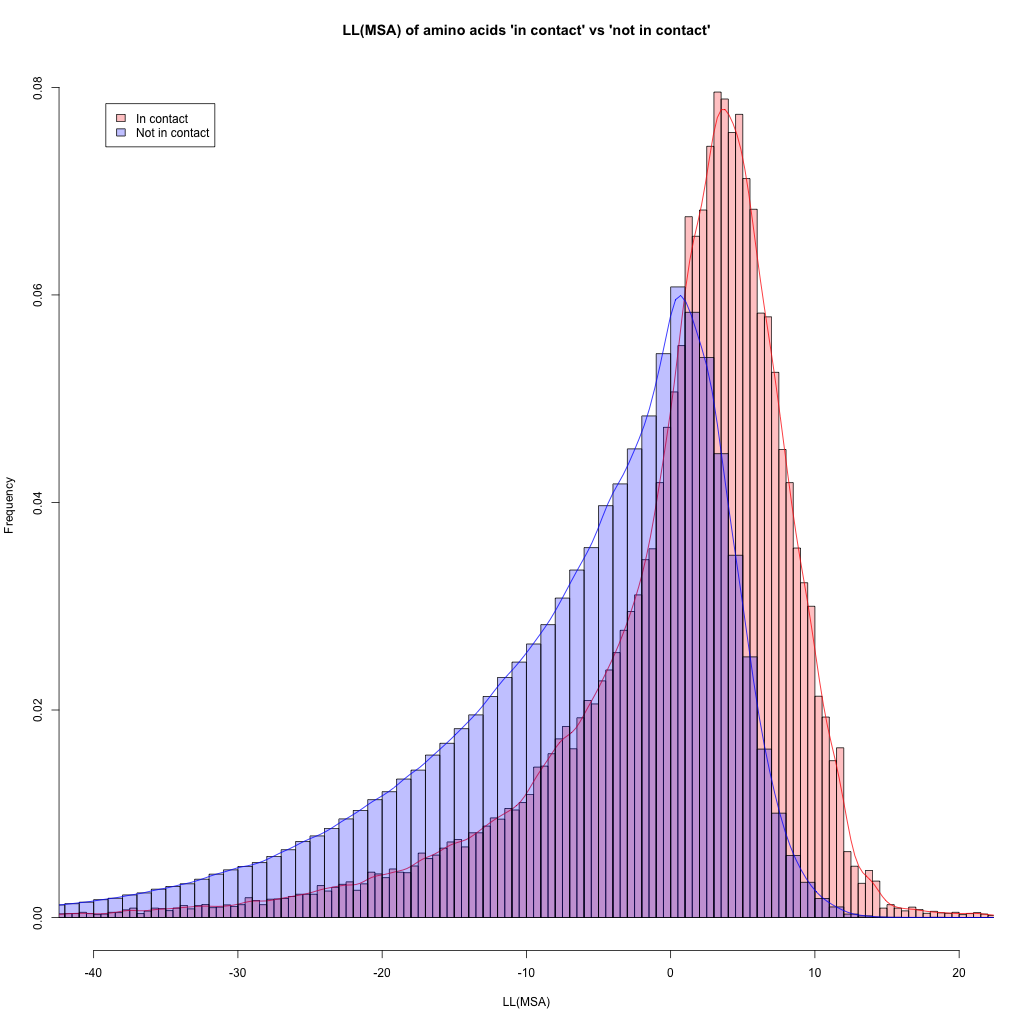
\includegraphics[width=10cm]{gwas_figure_2.png}
    \caption{LL(MSA) in contact vs ‘null’ within protein}
    \label{fig:gwasf2}
\end{figure}

We then computed $LL(MSA)$ to interacting amino acids from  different proteins. PDB ``compound molecule" structures were scanned and we defined: ``interaction", for amino acids whose atomic distance is 3 Angstrom or less, and ``null" (i.e. non-interacting) for distances of 30 Angstrom or more. These empirical distributions, allow us to approximate of the log odds of the ``interacting" vs ``null" amino acids distributions as $log_{odds}(x) = log[P(LL(MSA|Q2) \ge x) / P(LL(MSA|Q) \ge x] = e^{\alpha x}-\beta$ where $\alpha = 0.195$ and $\beta = 1.018$. The log odds value is capped to 4.0 to avoid artificially increasing Bayes Factors. As shown in figure \ref{f:}, the distributions of $LL(MSA)$ values are separated for ``null" and ``interacting" amino acids. 

\begin{figure}
    \centering
    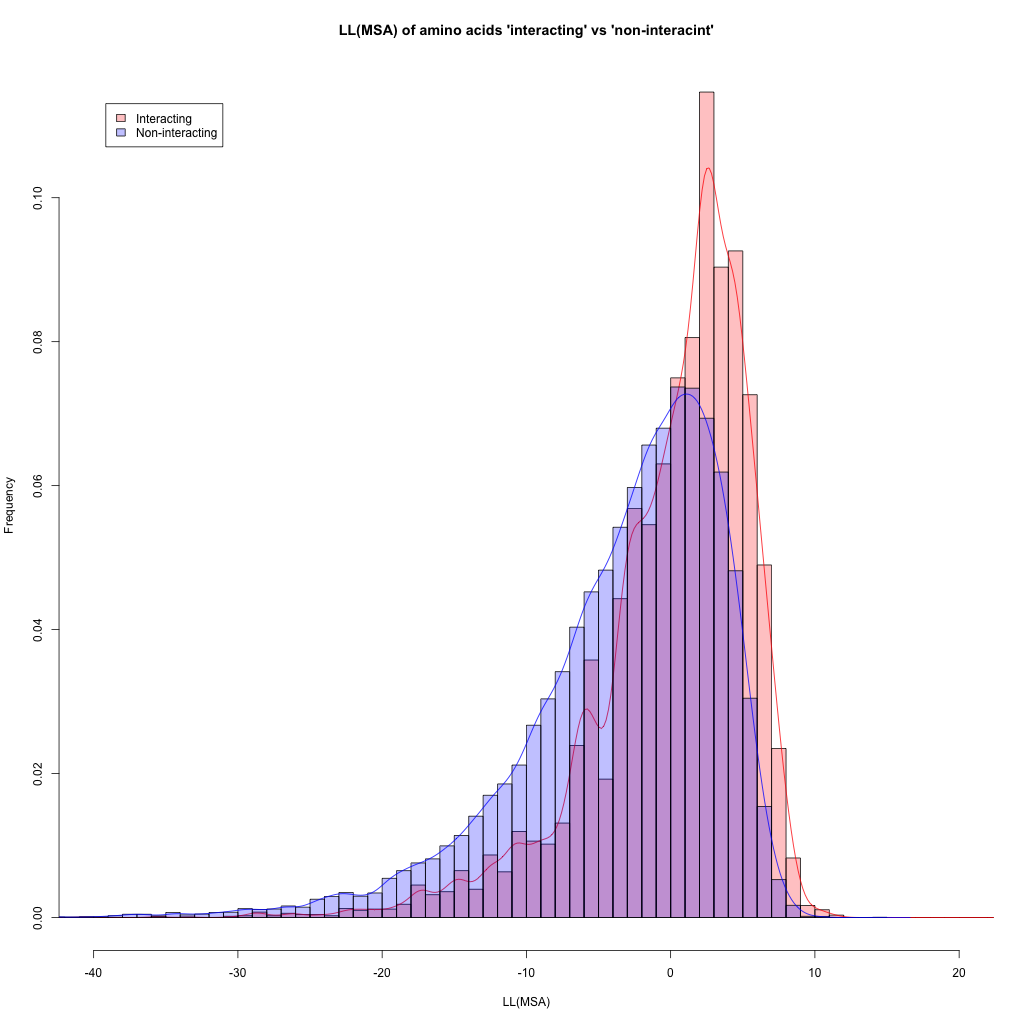
\includegraphics[width=10cm]{gwas_figure_3A.png}
	\caption{A) LL(MSA) in contact vs ‘null’ interacting amino acids in co-crystalized proteins (from Pdb), roughly 40\% of interacting records have $LL(MSA) > 1$. B) Log odds ratio of cummulative LL(MSA) probability (interacting / non-interacting).}
    \label{fig:gwasf3a}
\end{figure}
\begin{figure}
    \centering
    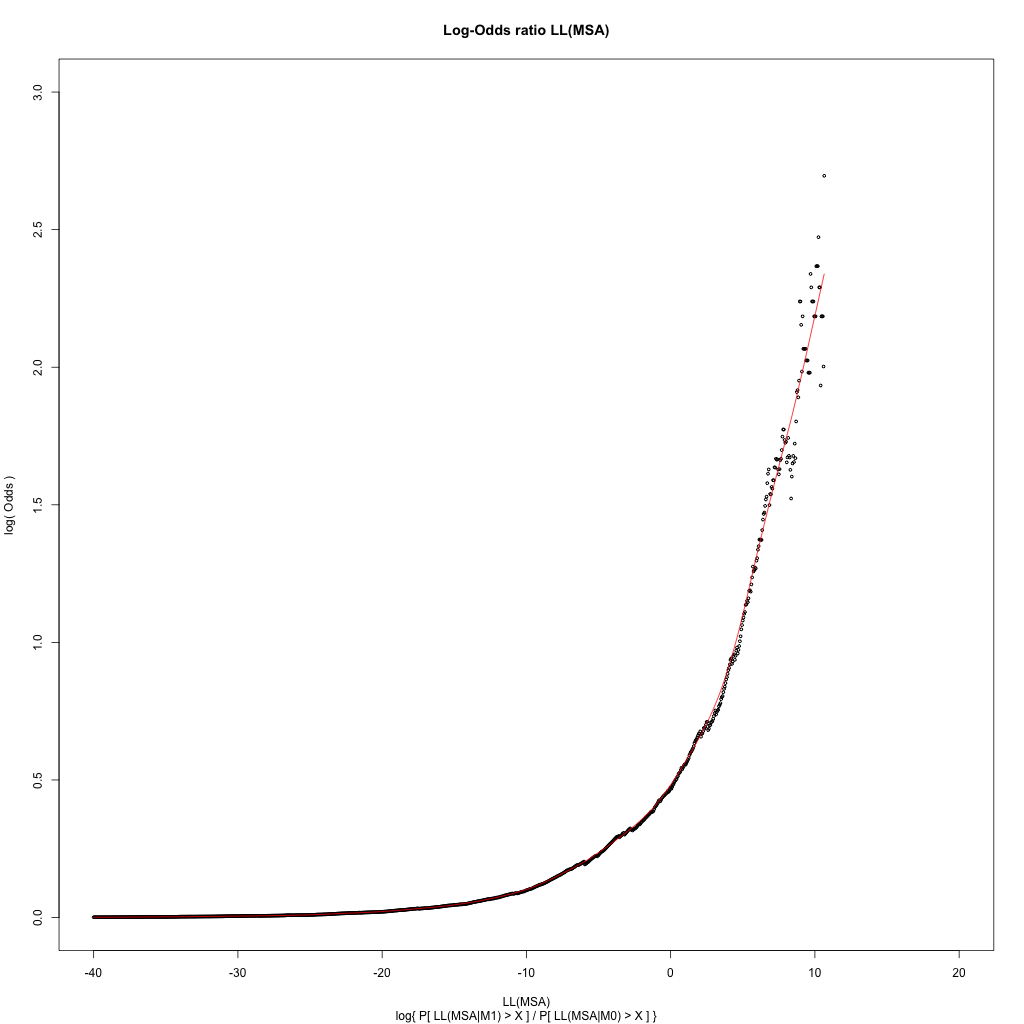
\includegraphics[width=10cm]{gwas_figure_3B.png}
    \label{fig:gwasf3b}
\end{figure}

Finally, we applied $LL(MSA)$ calculation to distinguish interacting genes. We define a set of ``interacting genes" as genes meeting three conditions: i) there is protein-protein interaction evidence (BioGrid \cite{stark2006biogrid}), ii) both genes are defined to belong to the same pathway (MsigDb, C2 groups \cite{subramanian2005gene}), and iii) both genes are expressed in the same tissue ( GTex \cite{lonsdale2013genotype}, expression of 1 FPKM or more, tissues $\in$ \{skeletal muscle, adipose tissue, pancreatic Islets\}). We define ``non-interacting" genes as those not fulfilling any of the three conditions.

We then calculate the average $LL(MSA)$ of three consecutive pairs of amino acids ($avg_3[LL(MSA)]$), either in the forward or reverse directions. For a given pair of genes, we calculate the highest $avg_3[LL(MSA)]$ and pick the highest number as representative for that pair. The distributions of genes in the ``interacting" set is higher than the distribution of the  ``non-interacting" genes (Supplementary Figure \ref{fig:S5}, $p-value < 2 10^{-42})$.

We also applied $LL(MSA)$ to separate clinically relevant variants from ClinVar database \cite{landrum2013clinvar} according to their clinical significance attribute (CLNSIG). We expect amino acids that may have ``compensatory mutations" to have high log-likelihood(MSA) within the same protein and be categorized as ``benign" (or druggable). Due to LD, ``compensated pairs" within proteins are more likely. As shown in Table \ref{t:}, different ClinVar categories have different distributions. As expected, benign variants have higher mean $LL(MSA)$ distribution than variants categorized as pathogenic or unknown (Supplementary Tables \ref{tab:S4A}, \ref{tab:S4B} and Figure \ref{fig:S4}).

\begin{figure}
    \centering
    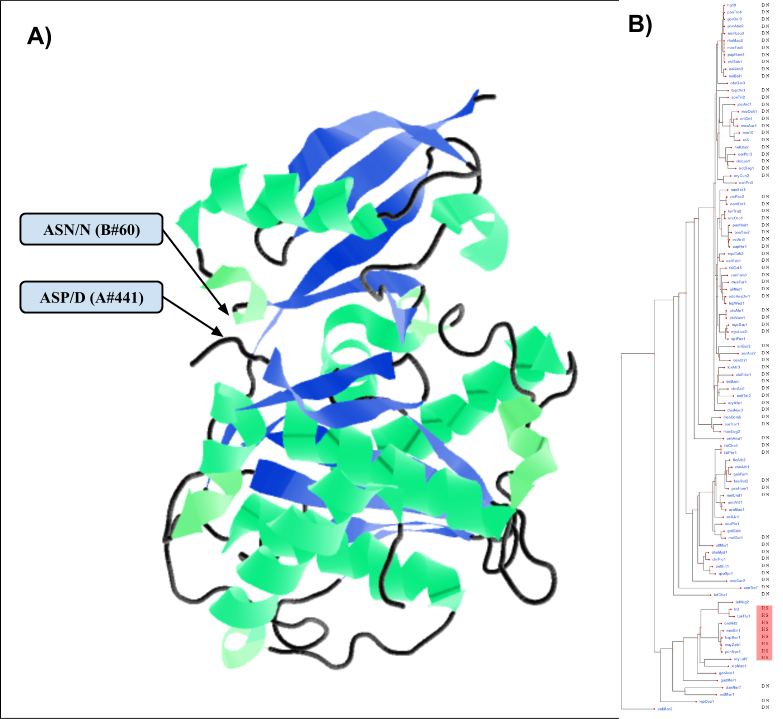
\includegraphics[width=14cm]{gwas_figure_jmol_epistasis.png}
	\caption{Example of amino acid interaction between SENP1 and SUMO1 proteins detected by out method $LL(MSA) = 7.7$. A) PDB structure 2G4D, shows that the amino acids are in close proximity: amino acid \#441 in SENP1 (ASP/D) interacts with amino acid \#60 in SUMO1 (ASN/N). B) Multiple sequence alignment and phylogenetic tree shows putative compensatory amino acid substitution pair ``D-N" replaced by ``H-S" (colors added for visual reference).}
    \label{fig:gwasf3a}
\end{figure}

\subsection{Epistatic GWAS analysis}

We run the epistatic GWAS analysis on a real dataset for Type 2 diabetes, consisting of over 13,000 samples and 1.2 million variants (detailed results to be published in a separate paper). The complete analysis takes less than 2 days using less than 1,000 CPUs in our cluster. This shows that an epistatic GWAS analysis of large cohort sequencing data is feasible using current computational resources.

%---
\section{Discussion}
%---

In this paper, we propose a novel methodology for genome wide analysis of variants located in putative epistatic sites. Due to the large number of statistical tests required in epistatic analysis, and the corresponding reduction of statistical power, this type of analysis is meant to be applied to datasets consisting of large number of samples which can overcome the reduction in statistical power. Our analysis methods have been optimized and parallelized to be suitable for large scale sequencing genomic studies.
We show the application of these methods to a large scale exome sequencing study for type II …..

